\chapter*{Introduction}
\addcontentsline{toc}{chapter}{Introduction}


\chapter{Document Classification}
    In this chapter we introduce a problem of document classification and commonly used approaches to this problem.
    \* % define what is document classification
    
    \section{Notation}
        This section provides a concise reference describing the notation and terms used in this chapter. 
        \* %add ore or move elsewhere
        
        \begin{table}[]
            \centering
            \begin{tabular}{c c}
                $D$ & Vocabulary. Denotes set (dictionary) of all used words in our dataset. \\
                $|D|$ & Size of the vocabulary. \\
                $tf_{w,s}$ & Number of times word $w$ appears in sentence $s$. \\
                $n_w$ & Number of times word $w$ appears in the whole corpus. \\
                $N$ & Number of documents in the corpus.
            \end{tabular}
        \end{table}
        
        Throughout this section we try to illustrate most things with examples. 
        For consistency, we will use following sample corpus of sentences and labels:
        
        \begin{table}[]
            \centering
            \begin{tabular}{c|c}
            \hline
                charlie is a good dog & 1 \\
                tiger is a bad cat & 0 \\
                oscar is a nice cat & 1 \\
                max is a bad dog & 0 \\
            \end{tabular}
            \caption{Example dataset}
            \label{tab:example:dataset}

        \end{table}
        

        This is an example pet sentiment dataset. Labels denote, if the statement was positive ($1$) or not ($0$).
        
        There are $1Q$ distinct words in the vocabulary $D$ of this corpus: 
        \begin{verbatim} a, bad, cat, charlie, dog, good, is, max, nice, oscar, tiger \end{verbatim}
        
        Later we will refer to them in this ordering, indexing from $1$. Hence $D_4=\mathrm{charlie}$.
    
    \section{Machine learning}
    
        \subsection{Supervised machine learning}
        Supervised learning is a standard approach in machine learning. 
        Supervised algorithms learn to predict the best outputs for a given input.
        We denote the collection of input data, features, as $X$ and the corresponding expected outputs, labels, as $Y$.
        $X$ is usually a matrix of real values where rows of this matrix are individual samples.
        $Y$ is usually a vector of real values or integers. 
        We refer to the pair of features and labels $(X, Y)$ as a dataset.
        
        Learning is usually done by optimizing parameters $\Theta$ of a parametrized function $f_\Theta$,
        with regards to a loss function $E_y(\hat{y})$. 
        We refer to function $f_\theta$ as a \textit{model}.
        Common loss is an $L2$ loss function $$E_y(\hat{y}) = \frac{1}{2}(y - \hat{y})^2 = \frac{1}{2}\sum_{i=1}^n (y_i - \hat{y})^2$$.  
        Formally we want to find parameter $\hat{\Theta}$ such that $\hat{\Theta} = argmin_\Theta \left(E_y(f_\Theta(x) \right)$. 
        This equation is usually not solved directly, but through an optimization process called learning \cite{Goodfellow-et-al-2016}. % deep learning book
        
        \subsubsection{Gradient descent}

        \textit{Gradient descent} method finds local minima of a usually multivariate function. 
        This is a well suited approach to use in context of supervised machine learning. 
        
        We use an observation, that if we follow the opposite direction of the function in a given point, 
        we arrive in a local minima. Example is on the picture \* %\ref{obr:gradient}.
        
        In a context of machine learning, we optimize a cost function $Q$ of parameters $\Theta$, 
        $$Q(\Theta) = E_y(f_\Theta(x))$$. We follow the opposite direction of gradient of the cost function $Q$ in respect to parameters $\Theta$. We initialize $\Theta_0$ to small random numbers and we perform an gradient descent step
        
        $$\Theta^{t+1} = \Theta^t - \alpha \frac{\partial Q(\Theta^t)}{\partial \Theta^t} = \Theta^t - \alpha \nabla Q(\Theta^t)$$
        
        $\alpha$ denotes the size of the step we will make and is commonly known as a learning rate. 
        We perform the gradient descent step until we are not improving enough any more. 
        Formally we stop, when $|\Theta^{t+1} - \Theta^t| < \epsilon$ for a given $\epsilon$ \cite{bottou-bousquet-2008}.
        
        This process is also sometimes refered to as a batch gradient descent.

        \begin{figure}
        \centerline{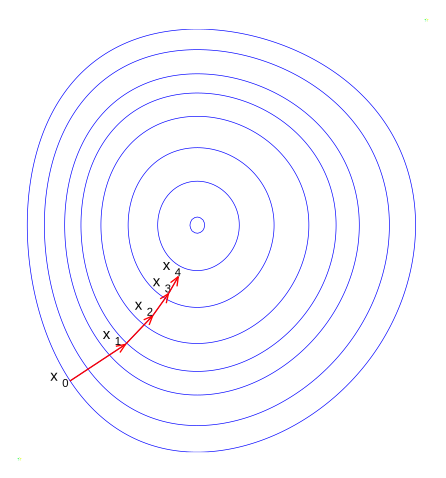
\includegraphics[width=0.4\textwidth]{images/gradient_descent}}
        \caption[Gradient descent]{Gradient descent \cite{pict} \*}
        \label{obr:gradient}
        \end{figure}
        
        
        \subsubsection{Stochastic gradient descent}
        
        During each gradient descent step, we need to go evaluate the gradient of the loss function over the whole dataset. 
        This is usually not feasible for larger datasets. 
        
        We can exploit the usual the cost function $Q$ can be rewritten as a sum of costs for each data point.
        
        $$Q(\Theta) = \sum_{i=1}^n Q_i(\Theta)$$
        
        $Q_i(\Theta)$ denotes the cost function computed on only the $i$-th element. 
        Finally we perform the gradient step for each example. 
        
        $$\Theta^{t+1} = \Theta^t - \alpha \frac{\partial Q_i(\Theta^t)}{\partial \Theta^t} = \Theta^t - \alpha \nabla Q_(\Theta^t)$$
        
        \* 
        For apropriate $\alpha$ we usually see a much faster convergence than for gradient descent.
        
        
        \subsection{Feed forward neural network}
        There is a lot of ways how to construct function $f_\theta$ that we want to optimize. 
        One of the most popular ones is roughly inspired by the human brain and is called a \textit{feed forward neural network}.
        
        Neural network consists of small interconnected computational units (neurons) that are usually organized into a layers.
        Each unit takes some inputs, based on them produces an output and sends it to other units. 
        In a feed forward neural network, the signal is always moving forward,
        hence unit on the $k$-th layer can only take it's input from previous layers \cite{Goodfellow-et-al-2016}.
        
        By adjusting the connections and theirs strengths, the network can learn to produce a specific output for a specific input.
        
        Simple neural network can be seen on an image \ref{obr:siet}.
        
        \begin{figure}
        \centerline{\includegraphics[width=0.4\textwidth]{images/siet}}
        \caption[Simple neural network with 2 layers, 3 inputs, 4 neurons and 2 outputs]{Simple neural network with 2 layers, 3 inputs, 4 neurons and 2 outputs\*} % redraw
        \label{obr:siet}
        \end{figure}
        
        The simplest model for a unit is weighted sum and application of some function. 
        Formally the unit receives a vector of inputs $x$ and computes output $g(\sum_{i=1}^n w_i x_i)$, 
        where $w_i$ is a connection strength to the $i$-th input.
        This one unit can be viewed as a simple one layer neural network with one output.
        
        Common realizations of function $g$ are: logistic function $g(x) = \frac{1}{1+e^{-x}}$, 
        hyperbolic tangent $g(x)=\frac{e^x-e^{-x}}{e^x+e^{-x}}$, relu $g(x) = \max(0,x)$ or leaky relu $g(x)=\log(1+\exp(x))$
        
        One layer of such units can be compactly described thanks to matrix notation as
        $$y=g(X W)$$
        
        $X$ represents the input matrix (number of samples $n$ times number of features $k$) and $W$ is the matrix of weights (number of features $k$ times number of units $u$). Note that function $g$ is applied element-wise.
        
        The important observation is, that we can chain such layers to from deeper neural networks.
        $$y=g(g(X W_1) W_2)$$
        
        $W_1$ are weight of hidden neurons and $W_2$ are weight of output neurons.
        There is no consensus in the community about how to count the layers. 
        For example the simple network on picture \ref{obr:siet} could be seen as a $3$ layer neural network,
        because it has input units, hidden units and output units.
        In this thesis we will use the number of matrices $W$ that crates the model.
        
        This family of functions is very broad and can in fact approximate any function \cite{cybenko1989approximation}.
        However, we need to train them first.
        
        \subsubsection{Back propagation}
        
        Back propagation is a method for effective computation of the gradient of a neural network.
        It relies on the the fact, that neural networks are just a simple compositions of matrix multiplications 
        and function applications. 
        It also relies on the fact, that functions used in the units are differentiable (almost everywhere).
        
        \textit{Back propagation} works in two parts, forward pass and backward pass.
        In the forward pass we feed to input to the network, compute activations of each layer and compute the final output.
        In the second pass, we make use of the chain rule and incrementally compute gradient with respect to each layer of the network.
        Then we use the gradient descent and optimize the parameters \cite{rumelhart1986david}.
        
        \* %example
        %Let's take for example the simple 2 layer neural network $y=g(g(X W_1) W_2)$ with the $L2$ loss. 
        %Let $h_1=g(X W_1)$. 
        %We need to compute $\frac{\partial Q(W_2)}{W_2} = \frac{E_y(g(h_1 W_2))}{\partial W_2}$. 
        %By using the chain rule we get 
        %$\frac{E_y(g(h_1 W_2))}{\partial W_2} = 
        %\frac{\partial E_y(\hat{y})}{\partial \hat{y}}\frac{\partial \hat{y}}{\partial W_2}$
        
    \section{Word and sentence representation}

        \subsection{Motivation}
        In order to apply machine learning techniques to a text classification, 
        we need to represent the text in a machine learning friendly way.
        Most machine learning algorithms expect the  input in a form of vectors of number. 
        
        Because of this, we need a system to translate string sentences $s$ into vectors $e$ of numbers. 
        Such vector is usually called an embedding. 
        
        In  other words, we need to project words and sentences into a vector space.
        
        \* % fix, that it is supervised vs unsupervised
        
        \subsection{Local representation}
        
        The simplest vector space is based on a local representation.
        In this representation, we use a vector space with $|D|$ dimensions, one for each word in the vocabulary.
        Value at the $i$-th position of the vector $v_i$ corresponds to a presence or an absence of the $i$-th words from the vocabulary, $D_i$.
        
        One of the simplest local representation is called a \textit{bag of words} (BOW). 
        In this representation, values in vectors are binary, where $1$ means that the word was present in the sentence and $0$ means it was not.
        Optionally we can extend this to a term vector, hence the number is not binary, but express the real count of given word in the sentence.
        
        Let's look at our example corpus. 
        Our vector space would have $10$ dimensions and the first sentence would be represented as a vector 
        $e = (1, 0, 0, 1, 1, 1, 1, 0, 0, 0, 0)$.
        
        This representation allows for simple sentence comparison. 
        Two sentences $s_1$ and $s_2$ can be compared via comparing cosine similarity of their BOW embeddings $e_1$ and $e_2$ as $\mathrm{sim}(s_1, s_2) = \mathrm{sim}(e_1, e_2) = \frac{e_1 e_2}{||e_1||.||e_2||}$.
        
        For technical reasons we can also define a cosine distance as 
        $$\mathrm{dist}(s_1, s_2) = \mathrm{dist}(e_1, e_2) = 1- \mathrm{sim}(e_1, e_2) = 1 - \frac{e_1 e_2}{||e_1||.||e_2||}$$.
        
        However this representation does not consider, that two words can be similar, even though they are not the same.
        For example words \texttt{nice} and \texttt{good} are consider completely different, even though they are not. 
        
        Second problem is, that this representation forgets the initial ordering of the words.
        This can be solved by using bigrams.
        
        Third problem is, that this representation assigns the same weight to each word.
        The fact that two sentences both has a meaningless word \texttt{a} has the same effect on the similarity as 
        if they both have word \texttt{good}. 
        This problem is partially solved by introducing term weights.
        
        \subsubsection{Term-weighting schemes}
        To emphasize that some words in the corpus are more important than other we introduce a weight Term-weighting schemes. 
        The idea is, that words like prepositions (\texttt{a}, \texttt{an}) and other words that are not very informative or redundant  (\texttt{is}, \texttt{do}, \texttt{by}) should should have smaller weights. 
        In practice, a list of \textit{stop words} is used to completely filter such words.
        
        Also words, that are to common in the dataset should have lower weight.
        If each sample is about a dog, we probably do not care about the word \texttt{dog}, because it is somehow redundant.
        
        However words, that appear multiple times in a sentence are probably important for this sentence and should have higher weights.
        
        Based on these two observations, a number of Term-weighting schemes was proposed \cite{salton1988term}.
        A Term-weighting schemes assign a weight to a word $w$ in a sentence $s$ as term weight $t_{w,s}$.
        These weights usually consists of two parts, \emph{term frequency} and \emph{inverse document frequency}. 
        
        \emph{Term frequency}, $\mathrm{TF}_{w,s}$, part reflects how important is word $w$ for sentence $s$.
        Common choices are:
        \begin{itemize}
            \item $\mathrm{sign}(\mathrm{tf}_{w,s})$, binary presence of the word in sentence. Also known as BOW.
            \item $\mathrm{tf}_{w,s}$, row number of appearances.
            \item $\frac{\mathrm{tf}_{w,s}}{|s|}$, number of appearances normalized by length of the sentence.
            \item $1+\log(\mathrm{tf}_{w,s})$
        \end{itemize}
        
        \emph{Inverse document frequency}, $\mathrm{IDF_w}$, part reflects how important is the word $w$ for the whole corpus.
        Common choices are:
        \begin{itemize}
            \item $1$, unary.
            \item $\log \left(\frac{N}{n_w} \right)$, inverse document frequency.
            \item $\log \left( 1+\frac{N}{n_w} \right)$, smoothed inverse document frequency.
            \item $\log \left( \frac{max_{w'} n_{w'}}{n_w} \right)$, max inverse document frequency.
            \item $\log \left(\frac{N-n_w}{n_w} \right)$, probabilistic inverse document frequency.
        \end{itemize}

        Note, that these choices for $\mathrm{TF}_{w,s}$ and $\mathrm{IDF}_{w,s}$ have probabilistically grounded \cite{aizawa2003information}. %information perspective on tfidf
        
        Another popular weighting scheme that is usually used in document retrieval is $\mathrm{BM_{25}}$. 
        
        $$\mathrm{BM}_{25~w,s} = \log \left(\frac{N-n_w+0.5}{n_w + 0.5}\right)    \frac{\mathrm{tf}_{w,s} (1.2 + 1)}{\mathrm{tf}_{w,s} + 1.2  \left(1 - 0.75 + 0.75 \cdot \frac{N}{\text{avgdl}}\right)}$$
        

        \subsection{Distributed representation}
        \cite{le2014distributed}


        \subsection{Prediction based distributedrepresentation}
        \cite{Rubenstein:1965:CCS:365628.365657} % distributional hyphotesis. 
        
        \cite{maas2011learning} % lda, vector space model

        \cite{DBLP:journals/corr/MikolovSCCD13} % podvzorkovanie.
        \cite{DBLP:conf/icml/LeM14} % slovne vektory
        \cite{rong2014word2vec} % some word2vec shit
        \cite{pennington2014glove} % glove word vectors


        \subsection{Count based distributedrepresentation}
        \cite{wiemer2004latent} % Latent semantic analysis
        \cite{landauer1998introduction} % introduction to lsa
        Latent Dirichlet allocation
        Explicit semantic analysis
        Latent semantic analysis
        Hierarchical Dirichlet process
        Non-negative matrix factorization
        \subsubsection{SVD}
        {$$
\begin{matrix} 
 M &  ~~ U & \Sigma & V^T \\
 \textbf{t}_j^T &  & &  \\
 \downarrow &  & &  \\
(\textbf{d}_i) \rightarrow 
\begin{bmatrix}
x_{1,1} \dots  x_{1,n} \\
\vdots ~~~  \ddots ~~~ \vdots \\
x_{i,1} \dots  x_{i,n} \\
\vdots ~~~ \ddots ~~~ \vdots \\
x_{m,1} \dots  x_{m,n} \\
\end{bmatrix}
=
&
\textbf{u}_i \rightarrow
\begin{bmatrix} 
\begin{bmatrix} & \textbf{u}_1 & \end{bmatrix} \\
\vdots \\
\begin{bmatrix} & \textbf{u}_l & \end{bmatrix}
\end{bmatrix}
&
\cdot
\begin{bmatrix} 
\sigma_1 \dots ~~~ 0 \\
\vdots ~~~ \ddots  \vdots \\
0  \dots  \sigma_l \\
\end{bmatrix}
&
\cdot
\begin{bmatrix} 
\begin{bmatrix} \, \\ \, \\ \textbf{v}_1 \\ \, \\ \,\end{bmatrix} 
\dots
\begin{bmatrix} \, \\ \, \\ \textbf{v}_l \\ \, \\ \, \end{bmatrix}
\end{bmatrix}
\end{matrix}
$$}
        \subsubsection{Truncated SVD}
        \subsubsection{Iterated SVD}
            \cite{brand2006fast} % incremental svd

        
        \subsection{Relationship of prediction and count based representations}
            \cite{naili2017comparative} % wrf is this? some comparison
            \cite{levy2014neural} % word2vec as matrix factorization
            \cite{altszyler2016comparative} % lsa vs word2vec on samall corpora
            \cite{levy2015improving} % word2vec hacks in lsi
    
        \subsection{Making the prediction}
            \* % cite something
    
    \section{Other approached for document classification}
        Recurrent neurl networks,
        Character based recurent neural networs, 

\* %\cite{manning2008introduction} introduction to information retrieval

\chapter{Related work}
    \section{LSI with class knowledge}
        \subsection{Supervised LSI}
            \cite{sun2004supervised} %supervised lsi, discriminative basis

        \subsection{Sprinkling}
            \cite{chakraborti2007supervised} % Sprinkling
        
        \subsection{Supervised weights}
            \cite{wu2017balancing} % word weights, TODO read
            \cite{ji2013discriminative} % TF KLD
            \cite{deng2014study} % supervised weights
            \cite{lan2009supervised} % supervised weights for text categorization

    
    \section{SVD in neural networks}
        \subsection{SVD as structured layer} 
            \cite{ionescu2015training} % svd in neural networks

    
\chapter{Our approach}
    \section{Goals and motivation}
    \section{Design}
    \section{Implementation}
        \cite{bird2009natural} % nlp in python
        \subsection{gensim lsa}
        \subsection{tensorflow for clasifier?}
    \*

\chapter{Experiments and evaluation}

    Performance
    
    Result analysis
    
    Weight analysis
    
    Transfer learning?

    \section{Classification datasets}
        \subsection{all datasets}
            \cite{conneau2017supervised} % datasets, benchmarks

    \section{Interpretability}
        \cite{ribeiro2016should} % explainability


